\documentclass[thesis.tex]{subfiles}
\begin{document}
\chapter{App Stores and App Preferences}
\label{chap:apps-and-stores}

Apps and app stores are a key part of the mobile ecosystem, an app being the key
form of software and the app store as their primary mode of distribution. In
this chapter we explore the stores and the policies surrounding them. We compare
the differences in terms and conditions between the various marketplaces and
make comparisons between them. We look at how users have privacy preferences
about the which apps they want to use, but by using AppPAL versions of common
user privacy preferences show how Android users do not seem to follow them in
practice. Finally we describe how AppPAL can be used to create new app stores by
checking for apps that can be shown to follow a policy, and offering them in a
web app-based store.

\section{App Stores}

Whilst iOS has just one store (Apple's App Store), the Android ecosystem is more
diverse with multiple stores available for multiple different purposes. The
dominant app store on Android is Google Play. Unlike iOS, Google isn't the sole
app vendor however. Some device vendors add their own stores to their devices as
a feature: Amazon do this with their Kindle Fire tablets, where Kindle owners
can download discounted apps. Some vendors, such as Samsung, add their own store
this to highlight apps that use features specific to their phones (KNOX in
Samsung's case). In some regions (such as China), using Google services is
problematic. People in these countries use local, regionally focused app stores
(such as QiHoo360 or Yandex) instead.

For a manufacturer to install Google's store they must comply with the Android
\ac{CDD}~\cite{google_android_2016}. The \ac{CDD} describes how to configure the
Android operating system and what features a device must have to run Android. If
a manufacturer cannot pass the \ac{CTS} that tests conformance with the \ac{CDD}
then they cannot install the Play Store.

For manufacturers like \emph{Jolla} whose devices do not run
Android\footnote{They run Sailfish, which is based off of the Linux Foundation's
Mer operating system.}, but can emulate some parts of the Dalvik virtual machine
enough to run Android apps, third-party stores like Yandex and Aptoide allow the
device to still benefit from apps designed for the Android ecosystem, without having to pass Google's test suites.

In this section we will focus on five different app stores: Apple's App Store,
Amazon's app store, Aptoide, Google Play and Yandex. Apple's App Store is for
iOS, but the rest are for Android operating systems. Amazon's app store was
opened in 2011 and was the primary app store for Amazon's Android-based Kindle
tablets\footnote{The Kindle Fire models, as opposed to the regular Kindle
models.}. Like Apple and Google's stores, the store is controlled by the device
manufacturer.

Yandex is a store primarily for the Russian and eastern European markets. It
features many Russian language apps. Some manufacturers, such as Nokia,
installed Yandex over Google's app store on devices sold in Russia.

Aptoide is a an open-source app store, and software for creating new app stores.
Unlike many other app stores it provides specialized app stores targeted for
Android based Smart TVs (Aptiode TV), and for users with slow internet
connections (Aptoide Lite). Aptoide doesn't provide access to fixed sets of
apps. Any user, or developer, is free to create their own \emph{curated}
repository of apps, and point Aptoide to it. Aptoide claim users and developers
have created over 220,000 stores using Aptoide. Notably the F-Droid app store
which sells only open source apps was created from a fork of Aptoide's code.
Aptoide tries to detect malware in its own repositories
(\autoref{fig:aptoide-malware}), like many other store vendors. Unlike others
rather than removing the malware Aptoide alert their customers that the app may
be dangerous. Not all apps are subject to these checks however. Searching the
store it was quickly possible to find an app designed to root
phones~(\autoref{fig:aptoide-root})

We chose these stores to focus on as they represent a range of different app
stores. From the largest of marketplaces (Apple and Google) to smaller
markets for specific devices (Amazon) specific regions (Yandex) and for
companies and users looking to create their own stores for their own devices
(Aptoide).

\begin{figure}
  \centering
  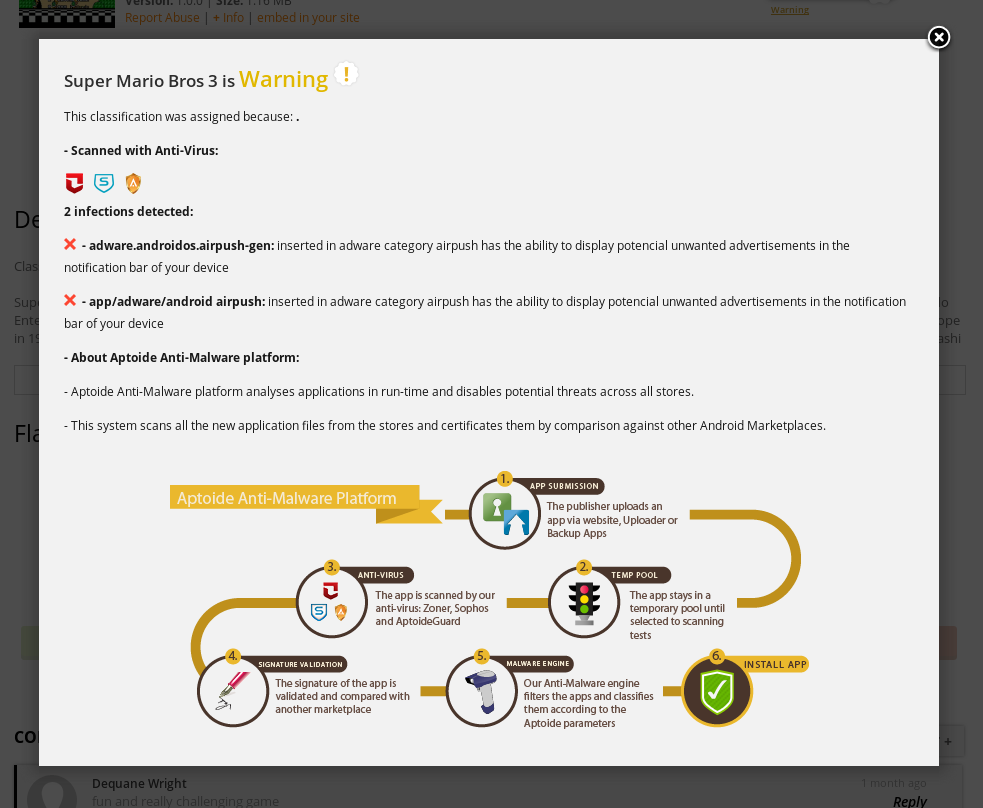
\includegraphics[width=0.8\linewidth]{figures/aptoide-malware.png}
  \caption{Adware infested and pirated app from Aptoide.}
  \label{fig:aptoide-malware}
\end{figure}

\begin{figure}
  \centering
  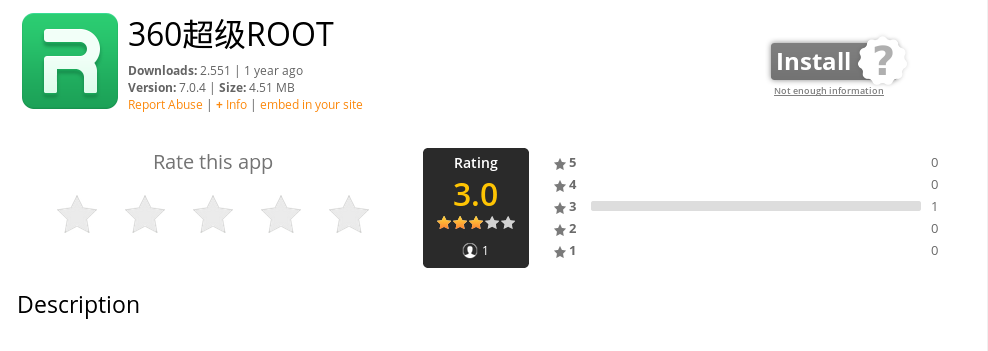
\includegraphics[width=0.8\linewidth]{figures/aptoide-root.png}
  \caption{Rooting app found on Aptoide.}
  \label{fig:aptoide-root}
\end{figure}


\subsection{Exploring Differences in Terms Between App Stores}

With the various app stores available, a user or developer might be
interested in the differences between the app stores.  Different stores require
different amounts of identification from their users to buy and sell
apps, or offer different terms and conditions.

The precise terms for using these app stores are hidden in user and
developer agreements.  The agreements hide within pages of legalese what the
stores are \emph{contractually} allowed to do with a user's data and a
developer's app.

A comparison of the terms and conditions is given in
\autoref{tab:terms-and-conditions}. It is also worthwhile comparing the forms
the terms and conditions themselves take. For most of the stores the terms are
single files or web pages written in English easily accessible from the store
homepages~\cite{yandex_yandex.store_nodate,aptoide_aptoide_nodate,google_google_nodate,amazon_amazon.co.uk_nodate}.

Apple's terms documents are split into many files and websites, and it is not
immediately clear how each document is related. The user agreements for all app
software and hardware are kept on one site in hierarchical menus with each
product, version of a product, and for each country appearing to have a separate
terms document. In practice many products share the same linked contracts,
within a single country. Developer terms and agreements are kept in a different
website and presented as a list of eleven policies. The iTunes terms and
conditions, which form the bulk of the agreements for using the iOS app store,
are also available in comic-book format ~\cite{r._sikoryak_terms_2017}.

\afterpage{{\tiny\sffamily\centering\raggedright
  \newcolumntype{R}{>{\raggedright\arraybackslash}p{0.13\linewidth}}
  \begin{longtable}{RRRRRR}
    \toprule
 & Apple & Amazon & Aptoide & Google & Yandex \\
    \midrule
    \endhead
    App User identification 
 & Apple ID.
 & Amazon account.
 & An ID and contact details.  User agrees not to give false ID. 
 & Name address and billing details.
 & For free apps no ID is needed, For paid apps they must be an \emph{authorized user} and give payment details
                                              \\\midrule
    Taken information
 & Technical data about the device, system, software and peripherals; which the Application Provider may use provided it is in a form that does not personally identify the user.
 & Device info, network connectivity, download info, location, usage info.  They will not access information unrelated to the app store.
 & Transaction information, which may be shared with developers.
 & App installation data (for malware identification), which may be opted out of.  Device ID, visited URLs and cookies.
 & Device info, OS info, device content, apps and services.  Mobile and SIM information.  Location (which can be denied), search queries and technical information.
                                              \\\midrule
    Payment info
 & Credit card or gift card.
 & Through Amazon.
 & Through an approved partner's payment processor.
 & Google Wallet, others at Google's discretion.
 & Through an approved processor provided by Yandex.
                                              \\\midrule
    Who pays whom?
 & The purchasing user pays Apple.  If a user uses \emph{family sharing} then the family organizer pays Apple.
 & User pays Amazon.
 & User pays the store owner through Aptoide.
 & User pays Google Commerce or the provider where Google is acting as an agent.
 & User pays the app supplier.
                                              \\\midrule
    Pricing
 & Apple sets price tiers which a developer may choose from.
 & Amazon, based on a minimum or suggested price from the developer.
 & The developer and store owners. Aptoide may round prices.
 & The developer.  Google may round prices.  If the developer makes an app free they may not charge later.
 & The supplier. The supplier agrees that Yandex may limit the exact amount of money and may convert to other currencies.
                                              \\\midrule
    Refunds
 & 14 days.
 & No.
 & 24 hours.
 & Only for defective or removed content.  A user may ask for a refund for 2 hours.  For an amount less than 10 USD a refund may be issued up to 48 hours later.  For amounts above 10 USD it depends on who processed the payment.
 & 15 minutes.
                                              \\\midrule
    Age of use
 & 13 or older to create an Apple ID.  Parents or guardians can create an ID through family sharing.  Educational institutions can create IDs for students.
 & Bellow 18 with consent of parent or guardian.  No alcohol content for under 21s.
 & A legal age within the user's country.
 & At least 13.  Bellow 18 with parent or guardian's consent.
 & At least 14.  Bellow 18 with parent or guardian's consent.
                                              \\\midrule
    Updates
 & Apple are not obliged to provide updates, and user's can chose not to install them.
 & By default they will be installed.
 & Aptoide can check for updates to apps and users will receive them.
 & Google will check for updates to apps and users will receive them.
 & Yandex may update content on devices for security and bug-fixing reasons.
                                              \\\midrule
    Moderation
 & Apple will moderate based on their own opinion of what is appropriate.
 & Publisher is obliged to give information which may be used to give ratings.  Amazon cannot check these ratings are correct.
 & Aptoide may review, screen, change and review apps but are not obliged to.  The Aptoide \emph{trusted app} sign indicates an automatic anti-virus checker checked the app and does not imply Aptoide checked it.
 & No obligation but Google may.
 & They may moderate and filter but are not obliged to.
                                              \\\midrule
    Rights to content
 & Apps are licensed to a user and not sold.  The user may use content on Apple devices.  If the device is later sold the user must remove the content.  The user may not distribute, copy, reverse engineer, disassemble, change or create derivative works with the licensed application or part thereof.
 & 
 & The user may not change, rent, lease, loan, sell, distribute or create derivative works based on the content.  The user may use the content.
 & The user cannot use apps as part of a public performance.  The user may transfer apps between linked Google accounts.  The user may not use content for dangerous activities, such as nuclear plants, life supporting, emergency communications, aircraft control or similar activities where failure might lead to death, injury and environmental damage.
 & 
                                              \\\midrule
      % Apple Amazon Aptoide Google Yandex
    What can the store do with the app?
 & Apple are appointed as the developer's agent/commissionaire to sell, market, and deliver apps. Apple may \emph{thin} an app, and repackage it for certain devices and optimization.
 & Irrevocable royalty-free right to distribute through all electronic means.  Amazon can check, test and store the app.  Amazon may change and add to the app for analytics, policy enforcement, to add metadata and to improve compatibility with Amazon devices.  They may, if requested by the developer add DRM.  Amazon may use the app to promote and advertise their services, and may make limited time promotions or \emph{test drive} versions of the app.  They may claim other rights.
 & Sell and make available to third-party stores.  They may change the app.
 & Google can reproduce, perform and display the app for marketing purposes.  Google may delegate this right to a third-party.
 & Yandex may use the app and developer's marks, logos and images of the app and its content worldwide.  Yandex may delegate or sub-license this right.
                                              \\\midrule
    How quickly will they remove an app at a developer's request?
 & No time period specified, but the developer may ask that they do it.  
 & 10 days generally.  5 days if due to a loss or third-party claim to rights.  ASAP if it is due to breaking the law.
 & No time period specified, but the developer may ask that they do it.
 & No time period specified, but the developer may ask that they do it.  If it is due to IP or breaking the law then users who downloaded within the last year can have a refund.
 & 90 days, though Yandex may keep an archive copy.
                                              \\\midrule
    Additional EULAs
 & The developer may add one, but it may not be inconsistent with the minimal terms and conditions provided by Apple, and must comply with all applicable laws in the regions the app is sold.
 & The developer may add one if it doesn't interfere with Amazon's own terms.
 & Aptoide add a default one, but they suggest developers add one that supersedes it.
 & Developer may add one, else the user is granted the worldwide perpetual right to perform, display and use the product.
 & Developer must add one and it must include the right to the content worldwide (except for trials).
                                              \\\midrule
    Developer identification
 & Apple Developer ID.
 & Amazon account.
 & Email address.  Using the same email as used for a Google Play developer account may help speed the app review process.
 & Google account and payment info.
 & Email, company name, tax ID, addresses, country of residence, website, order email address, user support email address, urgent Yandex support email address, payment information, other \emph{reasonable information}, which they do not define further.
                                              \\\midrule
    Content restrictions
 & Described by a \emph{living document}~\cite{apple_app_nodate}, which Apple will change as new example come up.  Broadly they look for safety, performance, business, design and legal issues. They also are aware \emph{kids} use their store and want developers to think about them when submitting apps.  They will reject amateurish, cobbled together apps.  Apps that they believe to have content that is \emph{over the line} (they say \emph{``they will know it when they see it''}).  Attempts to cheat the system will lead to developers being banned. 
 & No offensive content, pornography, illegality, gambling with real currency, IP infringing, privacy infringing, copyright infringing, or content that would be illegal in which the country the app would be sold.
 & Nothing that displays or links to: illegal content, invasions of privacy, content that interferes with the services of others, hate or violence, IP infringement. Nothing that harms devices or personal data.  Nothing that has unpredictable network usage or has an adverse impact on a user's service charges or a carrier's network.  Nothing that creates a \emph{spammy user experience}.
 & No apps implementing alternate stores can be submitted to the store. No sex or violence, bullying, hate, impersonation, IP infringing, PII publishing (specifically credit or ID card information, or non-public contacts), illegal content, gambling, dangerous (malware or spyware), self-modifying or system interfering content. No unpredictable network use.
 & Content must be safe, free of defects, and described accurately.  Nothing disruptive to Yandex or malware.  Nothing illegal such as: child pornography, obscenity, nudity, sex, extremist, hatred, violent, discriminatory, defamatory, gambling, copyright infringing or other forbidden material.  Nothing that steals private information nothing that mimics system functionality.  Nothing that would require Yandex to open-source anything via copy-left.  No alternative marketplaces.
                                              \\\midrule
    Who describes the apps
 & Developer
 & Developer but Amazon may edit it.
 & Developer.
 & Developer.
 & Developer but Yandex may edit it.
                                              \\\midrule
    Who can distribute apps?
 & Apple.
 & Amazon, and regional subsidiaries.
 & Aptoide and third-party partners using Aptoide to create their own store.
 & Google.
 & Yandex and partners.
                                              \\\midrule
    What support must a developer give?
 & None, except what is in app's EULA.  The developer must acknowledge that they are solely responsible for maintaining their app (not Apple).
 & Must respond to users within 5 days.  Must respond to Amazon within 24 hours if Amazon deem issue \emph{critical}.
 & Aptoide will give users with the developer's contact information.
 & Developer must support their app and handle complaints.  Developer must respond within 3 days and to issues deemed urgent by Google within 24 hours.  Failure to do so will result in Google lowering your app's ranking, review scores, and removal.
 & Must give user with support via email or phone.  Must respond to users within 5 days.
                                              \\\midrule
    When do developers get paid?
 & Within 45 days of the last day of the month.  Minimum earned balance is either 10 USD or 150 USD, depending on the developer's bank's country.
 & Roughly 30 days after app was sold.
 & Roughly 30 days after the end-of-the-month of the purchase.
 & On the 15th of the following month via Google Wallet.  Minimum earned balance for local currency payout is 1 USD. 100 USD for wire transfer payouts.
 & 30 days after the end-of-the-month of the purchase.  Minimum earned balance for payout is 100 USD.  If less is earned in a month Yandex will store it without interest.
                                              \\\midrule
    What do developers get paid?
 & Roughly 70\% of the price, as specified by~\cite{apple_itunes_2017}.
 & 70\% of list price (minus card processing fees).
 & 75\% of revenue share after deduction of all transaction fees.  Other rates subject to agreement with Aptoide.
 & 70\% of payment by user.
 & 70\% of net revenue (minus transaction fees).
                                              \\
    \bottomrule
    \caption{Comparison of terms and conditions from five app stores.}
    \label{tab:terms-and-conditions}
  \end{longtable}
}}

Comparing the terms and conditions in
\autoref{tab:terms-and-conditions}, the stores are for the most part
rather similar.  Stores pay their developers a month in lieu.  A user
must be over 18 to use the store, unless their guardian permits it.
No store is okay with developers selling illegal or sexually explicit
material.  Most stores are going to record information about the
users who bought software from them.  One area where the stores do
differ is in terms of refunds---only Apple has a return period longer
than a few hours.  In the case of Amazon there is no right to a
refund, and for Yandex only 15 minutes.

Another area where they differ is the rights a store has to the apps they sell.
Amazon and Aptoide both have the right to alter the apps. This is important
because it changes the trust model for apps on Android. In Android the developer
who signs the app is responsible for updates and identified as the developer of
the app. Android will not let a user install unsigned apps\footnote{Normally.
There are exceptions for development.}. To modify an app, Aptoide and Amazon
must be able to re-sign the code, essentially taking on the role of vouching for
the apps integrity and, by implication, its safety and security. Whereas an app
from Google's marketplace would be signed by the developer who made it, the
Amazon app store signs the apps it sells. In theory, an app originally purchased
in the Google Play store could be updated by an app from the Yandex store (if
signed by the same key and the app was a later version). With Amazon's model
this is not possible as they sign the app with different key. In Amazon's case
this is especially confusing as Amazon manufacture their own Android tablets. To
access certain \emph{system} permissions Android requires that an app be signed
by the same key that signed the OS installation. In the Play store model Google
no third-party developer in their store would have access to that key, but in
the Amazon model they could (if they desired) distribute system apps for their
Kindle devices. Having a different signing model is not inherently wrong, but it
changes the trust assumptions associated with Android which a user may not
necessarily be aware of. We discuss this further in \autoref{ssec:signing}.

%\todo{
%  Describe how a developer may have preferences about which app store to submit to, and state these differences could be encoded in apppal.
%  Mention how that would allow greater clarity in determining differences in stores as apppal is clearer than natural language.
%}

The terms and conditions are dense technical documents. Yet despite their
intimidating nature, the differences between each app store agreement is often
small. By encoding the key differences into a formal language (such as AppPAL)
we can start to clarify the small distinctions then a developer or user can
choose the app stores they are happy to submit to based on the store's policies,
and a company could automate the enforcement of the policy. For example in the
case of refunds the differences in policy could be written as shown in
\autoref{lst:refunds}. The differences in support agreements is shown in
\autoref{lst:support}. Again the differences are small: only differing in the
number of hours developers have to respond and whether there is a need to
respond to issues from the store itself more urgently.

%   Refunds
% Apple    & 14 days.
% Amazon    & No.
% Aptoide    & 24 hours.
% Google    & Only for defective or removed content.  A user may request a refund for 2 hours.  For an amount less than 10 USD a refund may be issued up to 48 hours later.  For amounts above 10 USD it depends on who processed the payment.
% Yandex    & 15 minutes.
\begin{figure}\centering
\begin{lstlisting}
'apple' says 'maximum-purchase-hours' is(336).
'apple' says User:U canRequestRefund(Purchase:P)
  if U hasCompletedPurchase(P), 'maximum-purchase-age' is(N)
  where age(P) < N.

'aptoide' says 'maximum-purchase-hours' is(24).
'aptoide' says User:U canRequestRefund(Purchase:P)
  if U hasCompletedPurchase(P), 'maximum-purchase-age' is(N)
  where age(P) < N.

'google' says 'maximum-purchase-hours' is(2).
'google' says User:U canRequestRefund(Purchase:P)
  if P isFor(App:A), A isDefective,
     U hasCompletedpurchase(P), 'maximum-purchase-age' is(N)
  where age(P) < N.

'yandex' says 'maximum-purchase-hours' is(0.25).
'yandex' says User:U canRequestRefund(Purchase:P)
  if U hasCompletedPurchase(P), 'maximum-purchase-age' is(N)
  where age(P) < N.
\end{lstlisting}
\caption{AppPAL translations of app store refund rules.}
\label{lst:refunds}
\end{figure}

\begin{figure}\centering
  \begin{lstlisting}
'amazon' says Developer:D mustRespondWithinHours(Issue:I, 120)
  if User hasIssueWith(I, App), D hasCreated(App).

'amazon' says Developer:D mustRespondWithinHours(Issue:I, 24)
  if 'amazon' hasIssueWith(I, App), D hasCreated(App),
     I isCritical.
     
'google' says Developer:D mustRespondWithinHours(Issue:I, 72)
  if User hasIssueWith(I, App), D hasCreated(App).

'google' says Developer:D mustRespondWithinHours(Issue:I, 24)
  if 'amazon' hasIssueWith(I, App), D hasCreated(App),
     I isCritical.

'yandex' says Developer:D mustRespondWithinHours(Issue:I, 120)
  if User hasIssueWith(I, App), D hasCreated(App).
  \end{lstlisting}
  \caption{AppPAL translations of app store support rules.}
  \label{lst:support}
\end{figure}

Writing policies out in this way describes the informal terms and conditions
unambiguously. A computer could check compliance with the terms by evaluating
the policy in this form (assuming it was given sufficient information).

If we were to translate the entire app store terms and agreements we could build
a set of standard decisions that describe what app stores terms and conditions
talk about. The similarity between the different rules in \autoref{lst:refunds}
and \autoref{lst:support} suggests there are idiomatic patterns present in the
policies that could be captured and described. In \autoref{chap:byod} we look at
BYOD policies and identify decisions and idioms common to those policies on the
basis of an AppPAL description of the rules. Similar techniques could also be
applied to app store terms to clarify and describe the policies precisely; going
beyond the comparison of the text of the policies presented here.

\subsection{Why Who Signed the App Matters}
\label{ssec:signing}

Some stores may make changes to the apps they sell. For Android users this is
important as it changes the trust relationships around who can provide updates
and who developed the app. We will illustrate the decisions Android makes using
AppPAL.

To install an app Android requires it to be signed with a key to
identify the developer.

\begin{lstlisting}
'android' says App:A isAcceptable
  if A isSignedWith(Key),
     Key isValid.
\end{lstlisting}

The standard Android trust model says that the developer of the app should be the person that signed it.

\begin{lstlisting}
'user' says Developer:D hasMade(App:A)
   if A isSignedWith(Key),
      Developer isOwnerOf(Key).
\end{lstlisting}

When upgrading an app the upgrade is only accepted if the certificates match
(and the version number is higher). Additionally if two apps have been signed by
the same key, they will share the same process space (enabling them to share
memory) and be able to share code.

\begin{lstlisting}
'android' says App:A canUpgrade(App:B)
  if A isSignedWith(Key),
     B isSignedWith(Key),
     A hasVersion(V1),
     B hasVersion(V2),
     Key isValid
  where A > B.
  
'android' says App:A canAccess(Data:D)
  if D isOwnedBy(DataOwnerApp),
     A isSignedWith(Key),
     DataOwnerApp isSignedWith(Key).
     Key isValid
\end{lstlisting}

To submit an app to the Play Store Google require that the key the app was signed with must be
valid until 2033, and more generally they recommend keys are valid for at least
25 years. 

\begin{lstlisting}
'play-store' says App:A isAcceptable
  if A isSignedWith(Key),
     Key isValid
  where expiryDate(Key) > 2033.
\end{lstlisting}

If an app is re-signed by a store to alter an app then it loses the
relationships set up by its original key. The store must now provide (or
re-sign) updates for the app it sold.
If the new key is also used to sign other apps then the app
may leak (or take) information from other apps shared by the same key.
Assumptions that data is private to one particular app start to break down if
apps are re-signed.  The user's trust model must now become:

\begin{lstlisting}
'user' says Store:D hasSold(App:A)
   if A isSignedWith(Key),
      Developer isOwnerOf(Key).
\end{lstlisting}

This policy is equivalent to the user's original trust model (they rely on the
same decisions), but the meaning is subtly different. The key that signed the
app is no longer sufficient to identify the developer.

\section{Finding the Right Apps}

For a user, finding the right apps is tricky.  Users need to discover
which ones are not going to abuse their data.  This is difficult as it
isn't obvious how apps use the data each has access to (including data
generated by the app or data already on the device).  Consider a user
attempting to buy a flashlight app.  The Play store shows users a long
list of apps when they browse.  Clicking through each app they can
find the permissions each requests but not the reasons why each was
needed.  They can see review scores from users but not from tools to
check apps for problems and issues like SSL
misconfigurations~\cite{fahl_why_2012}.  If they want to use the app
at work will it break their employers rules for mobile usage?

App stores give some information about their apps; descriptions,
screenshots and review scores.  Android apps show a list of
permissions when they're first installed.  In Android Marshmallow apps
display permissions requests when the app first tries to access
sensitive data (such as contacts or location information).  In
general, research shows that users do not understand how permissions
relate to their device~\cite{felt_android_2012,thompson_when_2013}.
Nevertheless, the device user must make the decision which apps to use
and which permissions to grant.

Some apps are highly undesirable.  There are many \acp{PUP} being sold
for Android
devices~\cite{truong_company_2014,vanja_svajcer_classifying_2013}.
Employees are increasingly using their own phones for work and an
employer may restrict which apps their employees can use.  The IT
department may set a \emph{mobile device policy}---a series of rules
describing what kinds of apps employees can used and how---to prevent
information leaks.  Some users worry that apps will misuse their
personal data---sending their address book or location to an
advertiser without their permission.  Such a user avoids apps which
can get access to their location, or address book; so they may apply their own
personal, informal, security policies when downloading and running apps.

\begin{table}\centering\sffamily\footnotesize
\newcommand{\tabtitle}[1]{\textbf{\footnotesize #1}}
  \begin{tabular}{ r l l l l }
    \toprule
    \tabtitle{Policy}                 & \tabtitle{C} & \tabtitle{A} & \tabtitle{F} & \tabtitle{U} \\
    \midrule
    \texttt{GET\_ACCOUNTS}            & \xmark       & \xmark       & \xmark       & \xmark       \\
    \texttt{ACCESS\_FINE\_LOCATION}   & \xmark       & \xmark       & \xmark       &              \\
    \texttt{READ\_CONTACT}            & \xmark       & \xmark       & \xmark       &              \\
    \texttt{READ\_PHONE\_STATE}       & \xmark       & \xmark       &              &              \\
    \texttt{SEND\_SMS}                & \xmark       & \xmark       &              &              \\
    \texttt{ACCESS\_COARSE\_LOCATION} & \xmark       &              &              &              \\
    \bottomrule
  \end{tabular}
  \caption[Lin~\etal{} policies expressed as sets of permissions.]{Lin~\etal{} privacy preference policies expressed as sets of prohibited permissions.}
  \label{tab:lin-perms}
\end{table}

To what extent do users follow personal policies informally?  In a
study of 725 Android users, Lin~\etal{} found four patterns that
characterize user privacy preferences for
apps~\cite{lin_modeling_2014} demonstrating a refinement of Westin's
privacy segmentation index~\cite{harris_interactive_privacy_2002}.
Lin~\etal~identified four types of user.  The \emph{Conservative} (C)
users were uncomfortable allowing an app access to any personal data
for any reason.  The \emph{Unconcerned} (U) users felt okay allowing
access to most data for almost any reason.  The \emph{Advanced} (A)
users were comfortable allowing apps access to location data but not
if it was for advertising.  Opinions in the largest cluster,
\emph{Fencesitters} (F), varied but were broadly against collection of
personal data for advertising.  We wrote AppPAL policies to describe
each of these behaviors as sets of prohibited permissions, shown in
\autoref{tab:lin-perms}.  These simplify the privacy policies
identified by Lin~\etal~as we do not take into account the reason each
app might have requested each permission (we could write more precise
rules if we knew why each permission was requested).  Lin~\etal~used
Androguard~\cite{andrew_desnos_androguard_2012} as well as manual
analysis to find the precise reasons the app requested each
permission~\cite{lin_modeling_2014}.

To test the extent that users were following the policies we took
installation from a partially anonymized database of installed apps
captured by Carat~\cite{oliner_carat:_2013}.

The Carat data set was collected as part of a UC~Berkley and University
of Helsinki experiment to measure the energy usage of apps.  As part
of the experiment users of the Carat app allowed the app to collect
which apps were installed on their device.  The data set was anonymized
by replacing the app names with hashes of the apps package identifier,
and usernames with an increasing integer key.

We used John the Ripper~\cite{solar_designer_john_2013}, with a
database of known package names and hashes, mostly derived from the
Android observatory~\cite{barrera_understanding_2012}.  Using these
hashes we can discover which users have installed which apps, by
comparing the hashes in the Carat data set to the hashes of apps we
knew we can discover which apps users had installed.

The database has over 90,000 apps and 55,000 users.  On average each
Carat user installed around 90 apps each; 4,300 apps have known names.
Disregarding system apps (such as \texttt{com.android.vending}) and
very common apps (Facebook, Dropbox, Whatsapp, and Twitter) we reduced
the set to an average of 20 known apps per user.  To see some
variation in app type, we considered only the 44,000 users who had
more than 20 known apps.  Using this data, and the apps themselves
taken from the Google Play Store and Android
Observatory~\cite{barrera_understanding_2012}, we checked which apps
satisfied which policies.

\begin{figure*}
  \centering
  \subfloat[Advanced policy]{%
    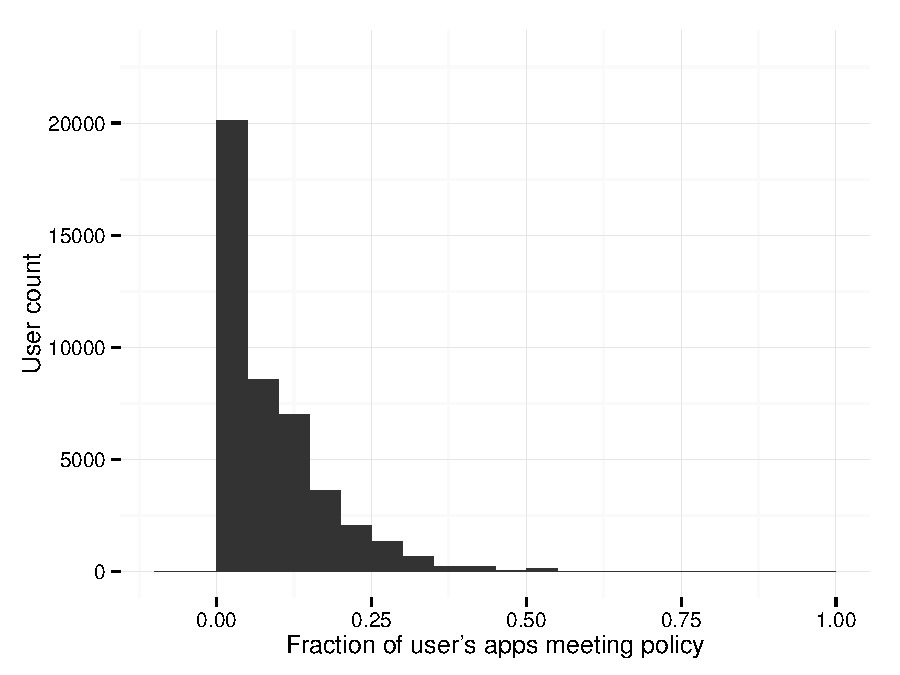
\includegraphics[width=0.45\linewidth]{figures/lin_a.pdf} 
  }
  \subfloat[Conservative policy]{%
    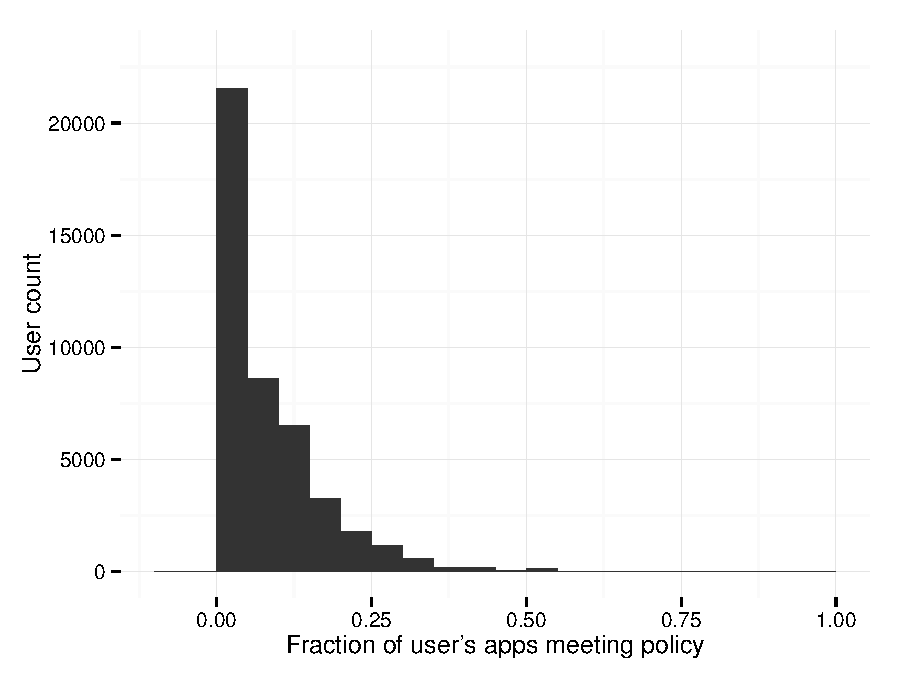
\includegraphics[width=0.45\linewidth]{figures/lin_c.pdf} 
  }\\
  \subfloat[Fencesitter policy]{%
    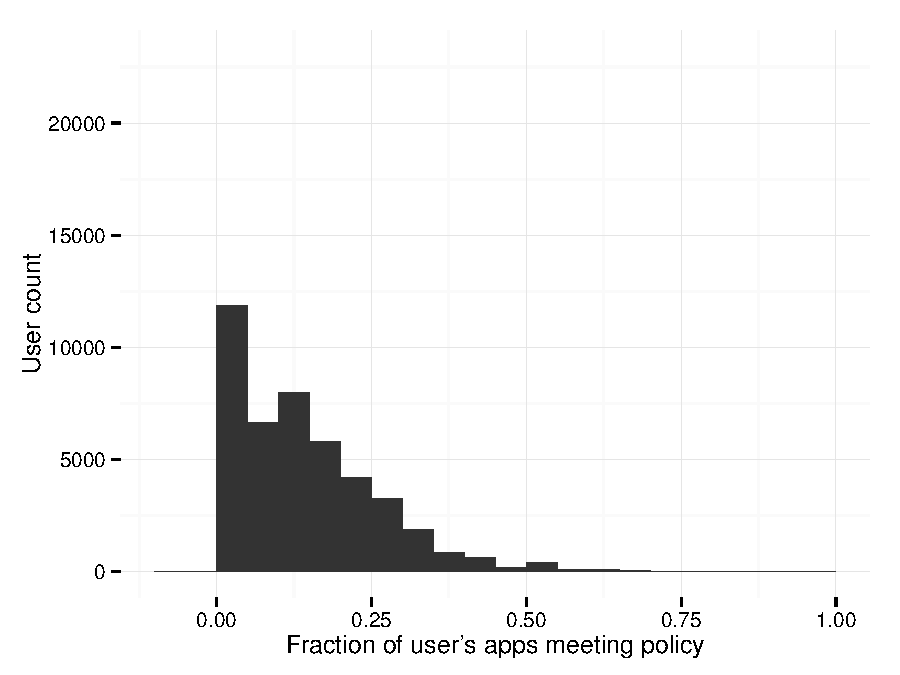
\includegraphics[width=0.45\linewidth]{figures/lin_f.pdf} 
  }
  \subfloat[Unconcerned policy]{%
    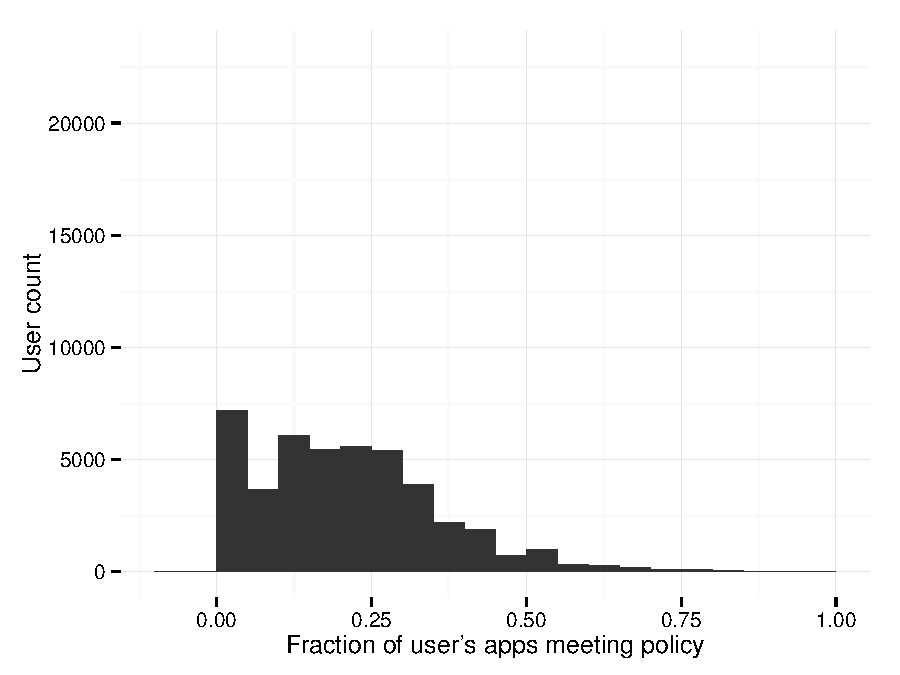
\includegraphics[width=0.45\linewidth]{figures/lin_u.pdf} 
  }\\
  \vspace{2em}
  \caption[Adoption of Lin~\etal~policies.]{Adoption of the four Lin~\etal~policies among users from the Carat data set.  Most users do not appear to follow these policies most of the time.}
  \label{fig:lin_uptake_graphs}
\end{figure*}

The charts shown in \autoref{fig:lin_uptake_graphs} show that very few
users seem to follow Lin~\etal's policies most of the
time. Even for the least onerous
\emph{unconcerned} policy, most users did not seem to follow the
policy most of the time.  This suggests that there is a disconnect
between user's privacy preferences and their behavior (reminiscent of
the \emph{privacy paradox}\footnote{The privacy paradox is that whilst
people will say they are very concerned about their privacy, they do
not alter their behavior to protect it.  It was first noticed by
psychologists looking at how people use social networks; though has
appeared in many other areas since.}); assuming the user population
studied by Lin~\etal~was similar to the data in the Carat study.

A few users, however, did seem to install apps meeting one of these
policies most of the time.  This suggests that while users may have
privacy preferences most are not attempting to enforce them.  This
suggests that policy enforcement tools, like AppPAL, may help users
enforce their personally desirable policies which they cannot do
easily using the current ad-hoc manual means available.

It is also interesting to discover when people install apps classified
as malware.  McAfee classify malware into several categories, and
provided us with a data set of apps classified as malware and
\acp{PUP}. Using these package IDs we calculated the package hashes
and looked to find users in the Carat data set who had installed any of
these apps.  The McAfee data classified the data into several
categories based on the purpose of the malware.  The \emph{malicious}
and \emph{trojan} categories describe traditional malware.  Other
categories classify \acp{PUP} such as aggressive adware.  Using AppPAL
we can write policies to differentiate characterizing users who allow
dangerous apps and those who install poor quality ones.

\begin{lstlisting}
'user' says 'mcafee' can-say
  'malware' isKindOf(App).
'mcafee' says 'trojan' can-act-as 'malware'.
'mcafee' says 'pup' can-act-as 'malware'.
\end{lstlisting}

If a user is enforcing a privacy policy we might also expect them to
be more selective about the apps they install.  If a user is being
selective we might expect them to install less malware and \acp{PUP},
as they often request many permissions. We can check this by using
AppPAL policies to measure the amount of malware each user had
installed.

\begin{figure}
  \centering
  \subfloat[Malware only]{%
    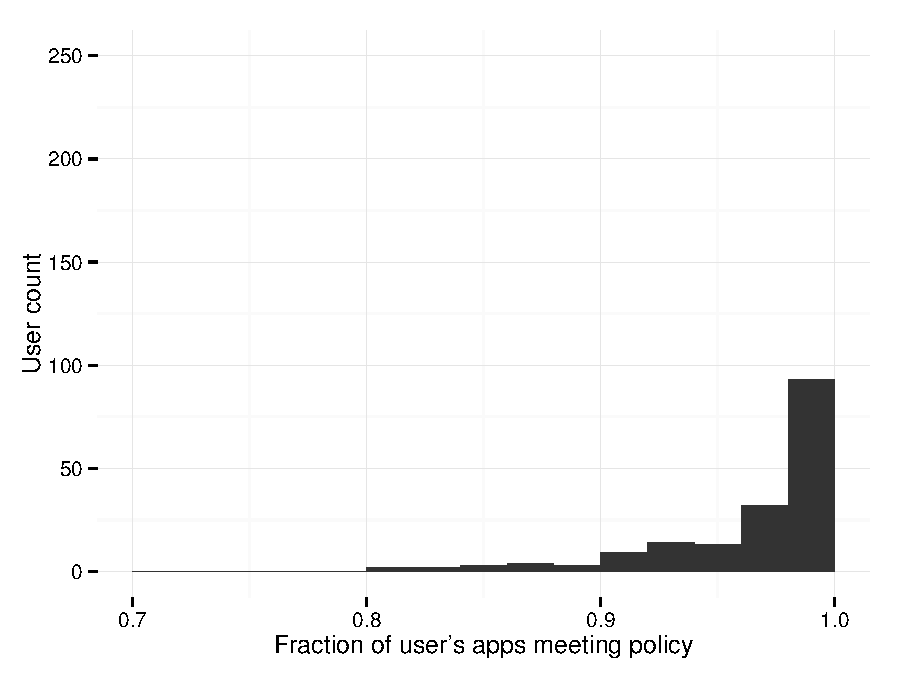
\includegraphics[width=0.45\linewidth]{figures/malware_np.pdf}
  }
  \subfloat[Malware and PUPs]{%
    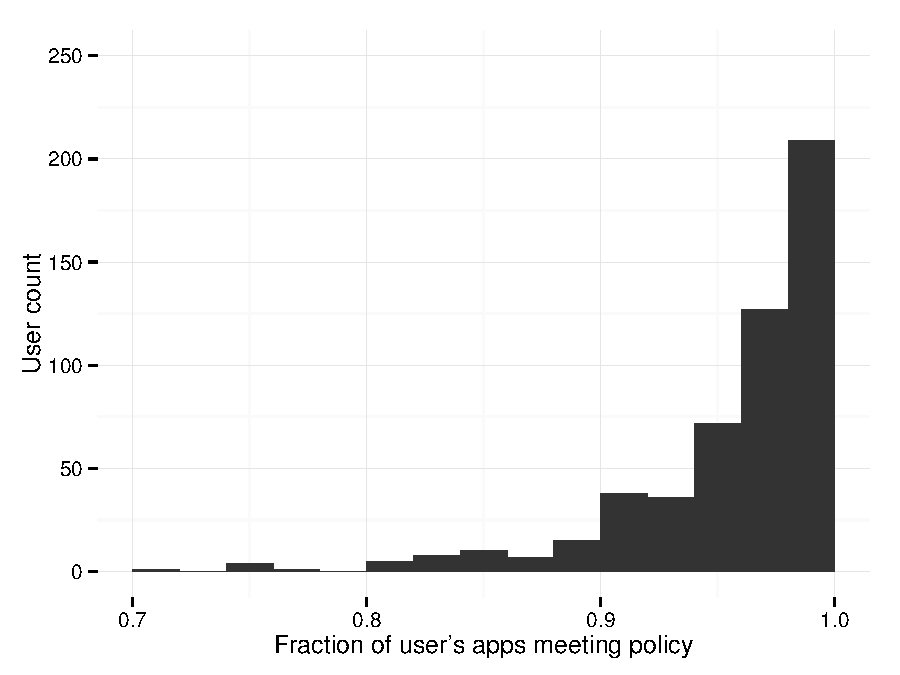
\includegraphics[width=0.45\linewidth]{figures/malware_nm.pdf}
  }\\
  \caption{Malware installation numbers in the Carat data set.}
  \label{fig:malware}
\end{figure}

We found that 1\% of the users had a \ac{PUP} or malicious app
installed.  Figure~\ref{fig:malware} shows that infection rates for
\acp{PUP} and malware is low; though a user is 3 times more likely to
have a \ac{PUP} installed than malware.  It is interesting to compare
a user's compliance to the Lin~\etal~policies with the amount of
malware each had installed (Figure \autoref{fig:lin_malware_graphs}).
Users who were complying more than half the time with the conservative
or advanced policies complied with the malware or \ac{PUP} policies
fully.  This suggests that policy enforcement is worthwhile: users who
do enforce policies about their apps experience less malware.  This
could also be attributed to the users selecting their apps more
carefully to enforce their policy: a careful user is unlikely to
install malware generally.


\begin{figure*}
  \centering
  \subfloat[Advanced policy and malware]{%
    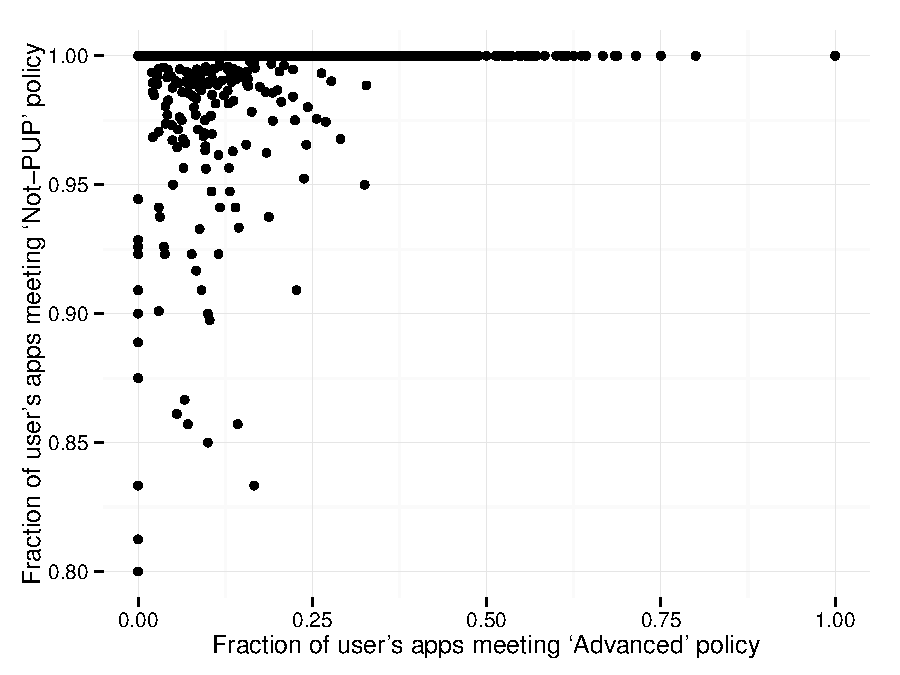
\includegraphics[width=0.45\linewidth]{figures/advanced-v-pup.pdf} 
  }
  \subfloat[Conservative policy and malware]{%
    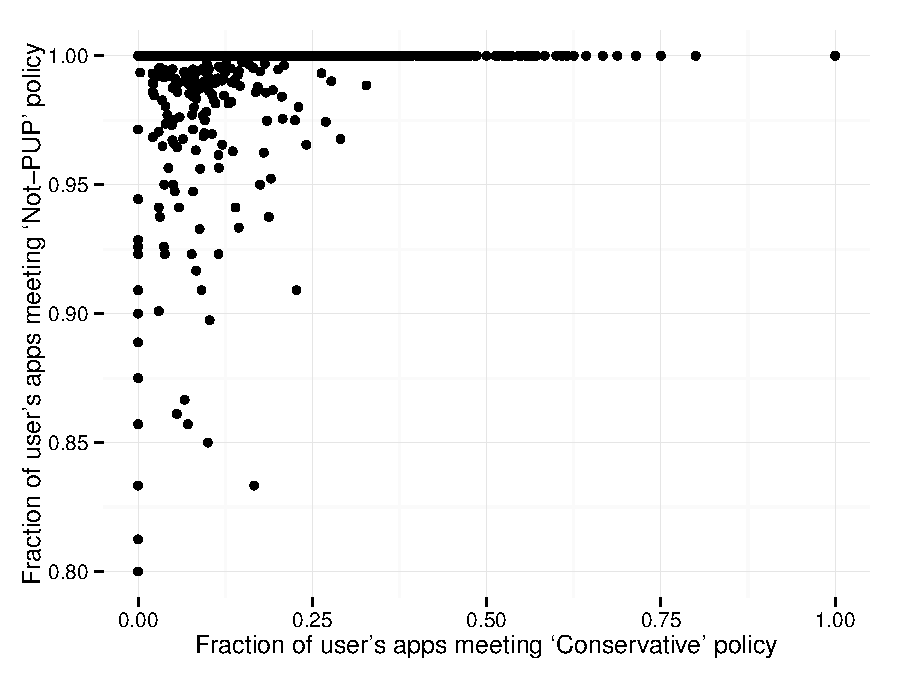
\includegraphics[width=0.45\linewidth]{figures/conservative-v-pup.pdf}
  }\\
  \subfloat[Fencesitter policy and malware]{%
    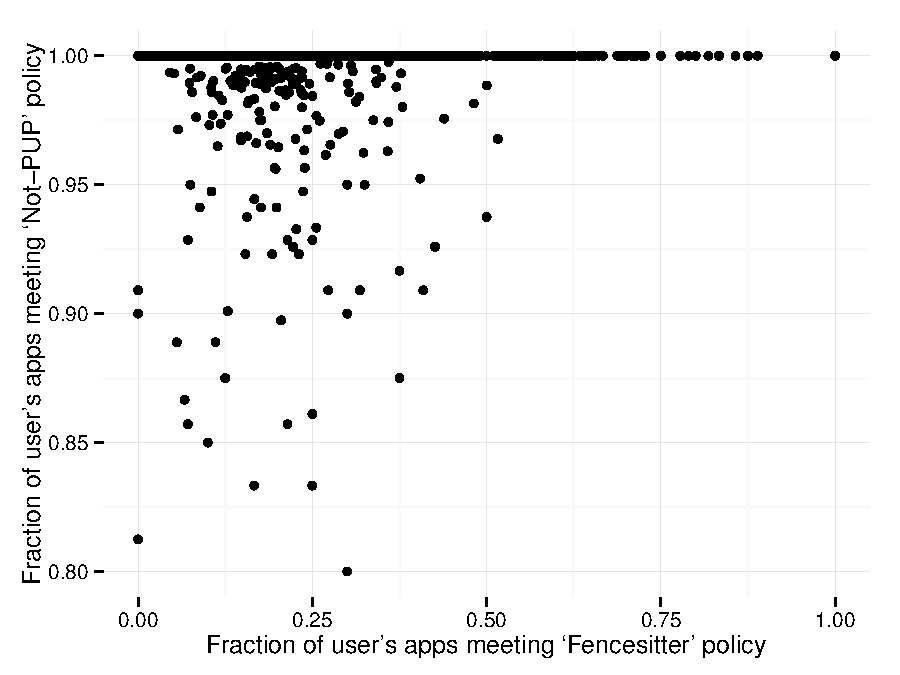
\includegraphics[width=0.45\linewidth]{figures/fencesitter-v-pup.pdf}
  }
  \subfloat[Unconcerned policy and malware]{%
    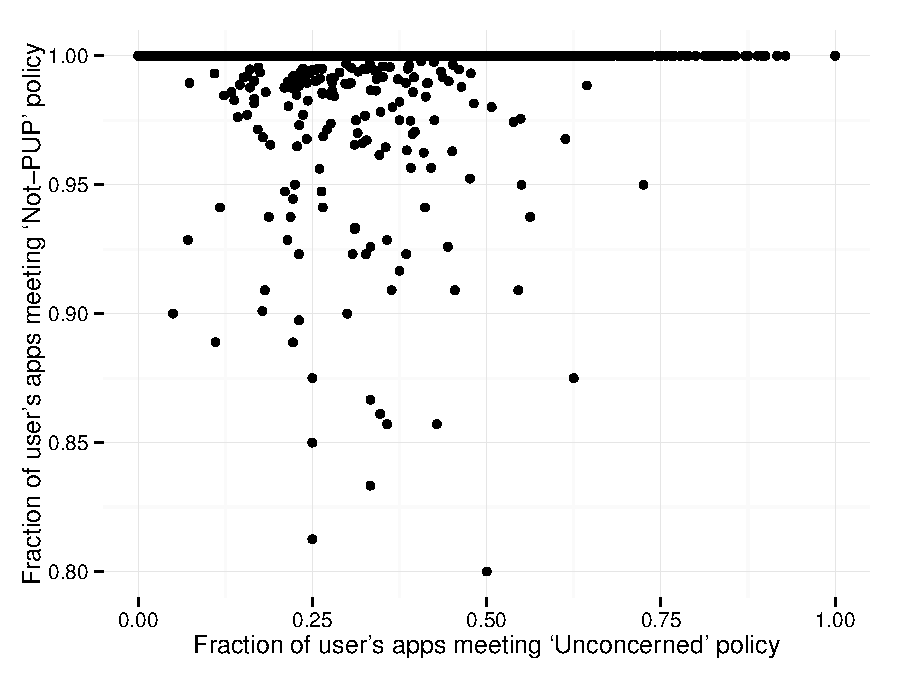
\includegraphics[width=0.45\linewidth]{figures/unconcerned-v-pup.pdf}
  }\\
  \vspace{2em}
  \caption[Plots of conformance to policies against malware installed.]{Graphs plotting a user's conformance with the Lin~\etal~policies against the amount of malware they had installed on their device.  Each dot represents a user.}
  \label{fig:lin_malware_graphs}
\end{figure*}


\section{An AppPAL Enhanced Store}

Using AppPAL we can describe users preferences for apps, and we can describe
the differences between some of the stores.  A natural continuation of this is
to start to generate new app stores, based on a user's policy, that only sell
apps that a user might find acceptable.

Curated app stores are a similar idea, used inside companies to help employees
install apps for work that satisfy company policies.  With these corporate stores the apps are hand selected
by IT staff.  

\begin{figure}\centering
  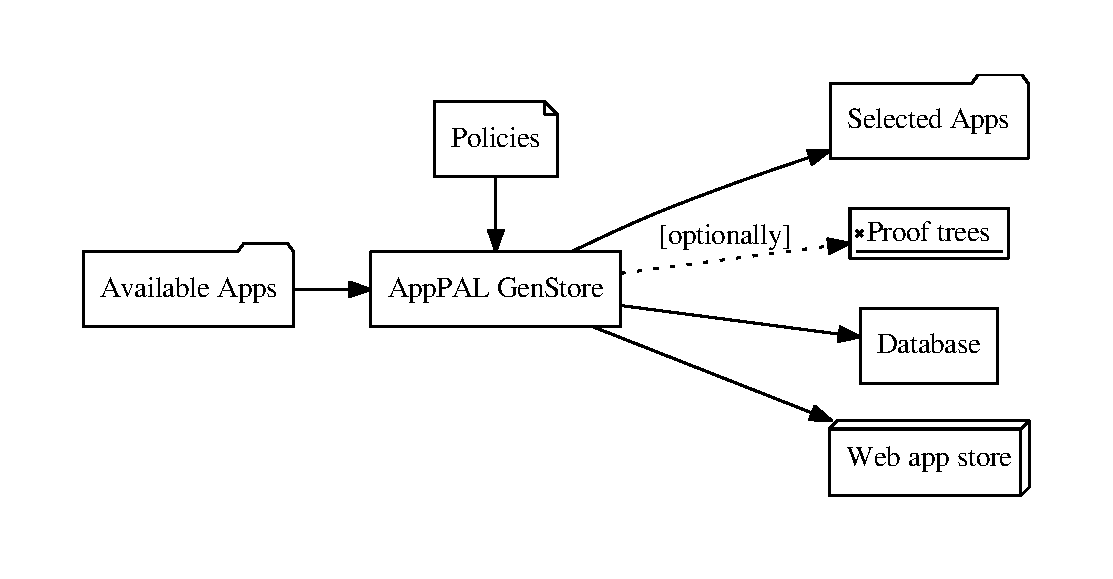
\includegraphics[width=0.8\textwidth]{figures/genstore.pdf}
  \caption[AppPAL GenStore's architecture.]{AppPAL GenStore's architecture.  In go policies and apps, out come app stores.}
  \label{fig:genstore-architecture}
\end{figure}

AppPAL's \emph{GenStore} tool automates this process for Android app stores. The
architecture is shown in \autoref{fig:genstore-architecture}. We summarize it
as:

\begin{enumerate}
\item The developer provides a pool of apps to GenStore. GenStore will select
  from among these apps to create the curated store.
\item The developer also provides a series of policy files. These should include
  rules to decide if an \emph{App isSellable}. Optionally they can also describe
  predicates where \emph{App hasCategory(Category)} which will be used to organize
  the apps into categories in the store.
\item GenStore runs, and for every app checks whether it is \emph{sellable}.
  Additionally it checks apps for each category (apps can belong to multiple
  categories), if defined. From this the GenStore builds a database
  (\autoref{fig:genstore-schema}) documenting which apps are available, their
  categories and some additional metadata.
\item A web-app is created from a template. The default template uses the Sinatra
  framework to serve the store, but any framework could be used. Alongside the
  web-app, Genstore copies the selected APK files into a directory and a database
  is created storing information about the apps.
\end{enumerate}

Genstore is a prototype, but it lets developers explore how policies could be
integrated into the Android ecosystem. It shows an example of how AppPAL can
help make decisions, in this case about which apps make the cut for a store,
automatically. For a company seeking to enforce a policy about which apps are
installable they could use it to offer their employees choice about apps,
without having to remove the default store entirely. If an AV vendor integrated
their own checks into AppPAL then they could create a \emph{safe} app
store where all apps have been demonstrably vetted by their software and
engineers.

\begin{figure}\centering
  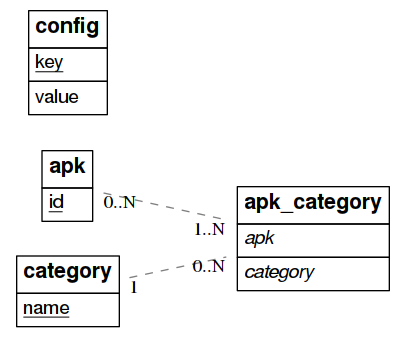
\includegraphics[width=0.4\textwidth]{figures/genstore-schema.png}
  \caption{GenStore database schema.}
  \label{fig:genstore-schema}
\end{figure}

%\begin{figure}\centering
%  \framebox[\textwidth]{TODO: ADD SCREENSHOT WHEN I FIX THE BUGS\vspace{3in}}
%  \caption{Screenshot of a generated store.}
%  \label{fig:genstore-screenshot}
%\end{figure}

\end{document}

%%% Local Variables:
%%% mode: latex
%%% TeX-master: "../ch4"
%%% End:
